%% LaTeX-Beamer template for KIT design
%% by Erik Burger, Christian Hammer
%% title picture by Klaus Krogmann
%%
%% version 2.1
%%
%% mostly compatible to KIT corporate design v2.0
%% http://intranet.kit.edu/gestaltungsrichtlinien.php
%%
%% Problems, bugs and comments to
%% burger@kit.edu

\documentclass[18pt]{beamer}
\usepackage[utf8]{inputenc}


%% SLIDE FORMAT

% use 'beamerthemekit' for standard 4:3 ratio
% for widescreen slides (16:9), use 'beamerthemekitwide'

\usepackage{templates/beamerthemekit}
% \usepackage{templates/beamerthemekitwide}

%% TITLE PICTURE

% if a custom picture is to be used on the title page, copy it into the 'logos'
% directory, in the line below, replace 'mypicture' with the 
% filename (without extension) and uncomment the following line
% (picture proportions: 63 : 20 for standard, 169 : 40 for wide
% *.eps format if you use latex+dvips+ps2pdf, 
% *.jpg/*.png/*.pdf if you use pdflatex)

\titleimage{Knot3}

%% TITLE LOGO

% for a custom logo on the front page, copy your file into the 'logos'
% directory, insert the filename in the line below and uncomment it

\titlelogo{nologo}

% (*.eps format if you use latex+dvips+ps2pdf,
% *.jpg/*.png/*.pdf if you use pdflatex)

%% TikZ INTEGRATION

% use these packages for PCM symbols and UML classes
% \usepackage{templates/tikzkit}
% \usepackage{templates/tikzuml}

% the presentation starts here

\title[]{\huge{Knot$^3$} }
\subtitle{Praxis in der Softwareentwicklung WS 2013/14}
\author{Tobias Schulz, Maximilian Reuter, Pascal Knodel, Gerd Augsburg,\\ Christina Erler, Daniel Warzel}

\institute{Institut für Betriebs- und Dialogsysteme, Lehrstuhl für Computergrafik}

% Bibliography

\usepackage[citestyle=authoryear,bibstyle=numeric,hyperref,backend=biber]{biblatex}
\addbibresource{templates/example.bib}
\bibhang1em

\begin{document}

% change the following line to "ngerman" for German style date and logos
\selectlanguage{ngerman}

%title page
\begin{frame}
\titlepage
\end{frame}

%table of contents
%\begin{frame}{Outline/Gliederung}
%\tableofcontents
%\end{frame}

\section{Das Spiel}
\begin{frame}{Knot$^3$}
Platzhalter
\begin{columns}[c]
	\column{.5\textwidth}
	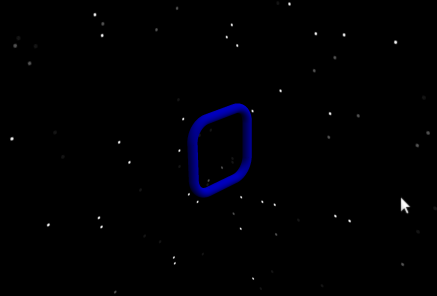
\includegraphics[scale=0.5]{simpelgeometry}
 	\column{.5\textwidth}
 	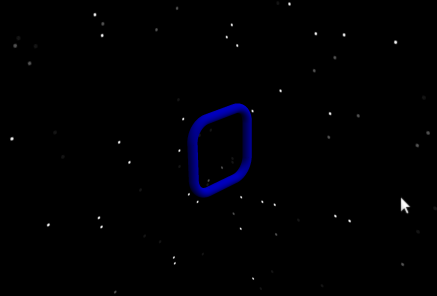
\includegraphics[scale=0.5]{simpelgeometry}
\end{columns}

\end{frame}


\subsection{Konzept}
\begin{frame}{Idee}
\begin{itemize}
\item kreatives Aufbau- und Knobelspiel
\item geometrisches Objekt verändern (Knoten)
\item eigene Aufgaben erstellen
\item intuitive Navigation
\end{itemize}
\end{frame}

%\begin{frame}{Konzeptzeichnung}
%\begin{center}
%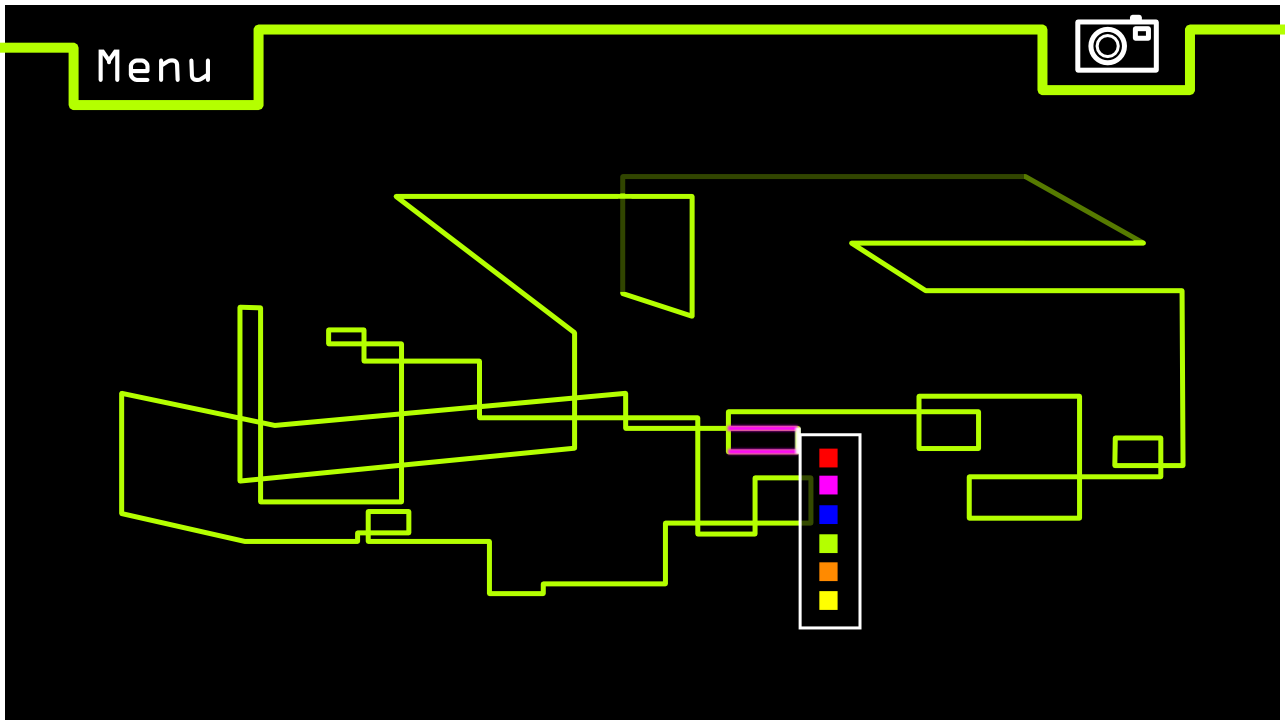
\includegraphics[scale=0.3]{mockup} \\
%Quelle: HfG - Greta Hoffmann
%\end{center}

%\end{frame}
%\begin{frame}{Pflicht-Vorgaben}
%\begin{itemize}
%\item Übersichtliche Darstellung
%\item Komplexe 3D-Geometrie mit Verdeckungen soll frustfrei %wahrnembar sein
%\item Intuitive Navigation
%\item Selektion und Modifikation von Kanten
%\item Übergehen unmöglicher Kantenzustände
%\item Highscores (in diesem Fall nach Zeit)
%\item Einfaches Datenaustauschformat
%\item Mindestens zehn eindeutige Levels mit steigendem %Schwierigkeitsgrad
%\end{itemize}
%\end{frame}

\begin{frame}{Möglichkeiten von Knot$^3$}
Platzhalter
\begin{columns}[c]
\column{.5\textwidth}
 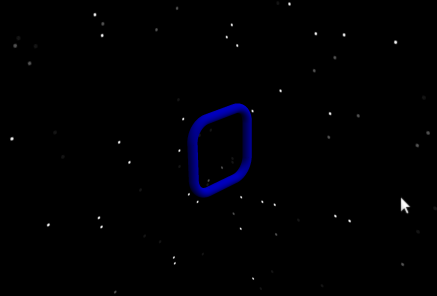
\includegraphics[scale=0.5]{simpelgeometry}
 \column{.5\textwidth}
 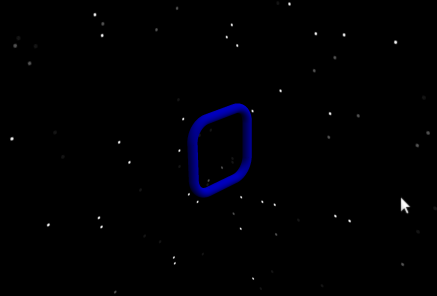
\includegraphics[scale=0.5]{simpelgeometry}
\end{columns}
\end{frame}

\begin{frame}{Was uns wichtig war}

\begin{columns}[c] 
    \column{.65\textwidth}
    \begin{itemize}
	\item Portierbarkeit auf Linux
	\item Soundeffekte
	\item Hintergrundmusik
	\end{itemize}
    \column{.35\textwidth}
    
\includegraphics[width=\textwidth]{linux} \\
    Quelle: papervisions.com
    \end{columns}
\end{frame}

\subsection{Marktanalyse}
\begin{frame}{Marktanalyse}

\begin{itemize}
\item Kein vergleichbares Spiel auf dem Markt
\item Es gibt bereits Werkzeuge zum generieren von Knoten, aber keines dieser Programme setzt auf ein Spielkonzept

\end{itemize}
\end{frame}

\subsection{Demonstration}
\begin{frame}{Demonstration}
\begin{center}
\Huge \textbf{Demo}
\end{center}

\end{frame}





\section{Zukunft}
\subsection{Vermarktung}
\begin{frame}{Vermarktung}
\begin{itemize}
\item Freeware
\item Sourcecode öffentlich (MIT-Lizenz)
\item Spiel und Sourcecode auf knot3.de

\end{itemize}

\end{frame}


\begin{frame}{knot3.de}
\begin{center}
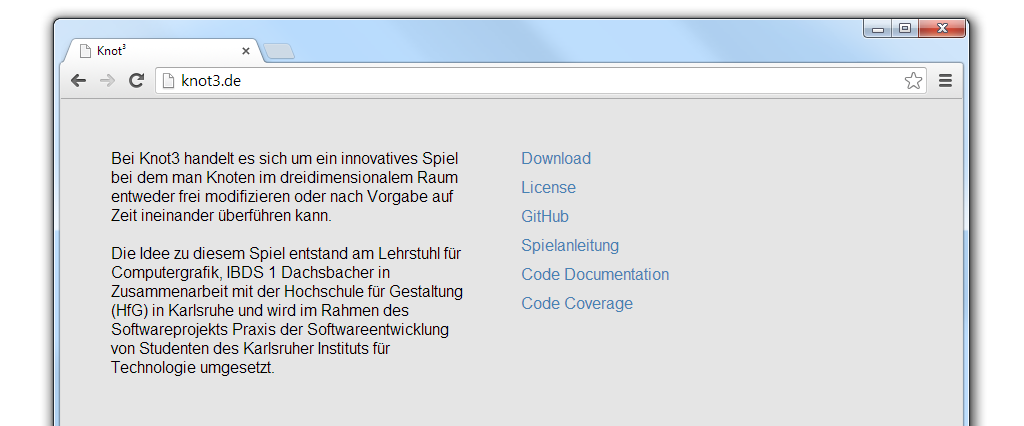
\includegraphics[scale=0.44]{webseite}
\end{center}

\end{frame}

\subsection{Weiterentwicklung}
\begin{frame}{Weiterentwicklung}
Was könnte noch kommen?
\begin{itemize}
\item MacOSX-Unterstützung 
\item Web-Version
\item Neue Spielmodi
\item Online-Datenbank für Levels
\end{itemize}

Durch die MIT-Lizenz ist es jeder Person ermöglicht dieses Projekt nach ihren Vorstellungen zu verbessern.
\end{frame}

\section{Fakten}
\subsection{Statistik}
\begin{frame}{Statistik}
\begin{itemize}
\item 6 Entwickler
\item 27391 Codezeilen (Stand 19.03.14)
\item 183 Klassen
\end{itemize}
\end{frame}

\subsection{Herausforderungen}
\begin{frame} {Herausforderungen}
Einarbeitung und Erlernen von:
\begin{itemize}
\item C\#
\item XNA-Framework / Mono-Framework
\item Cross-Platform-Entwicklung
\item Programmierung von 3D-Anwendungen
\item Teamarbeit und -koordination
\item Kollaboration mit Git
\end{itemize}
\end{frame}


\section{Fragen}
\begin{frame}{Fragen}
\begin{center}
\Huge \textbf{Weitere Fragen?}
\end{center}
\end{frame}



%\appendix
%\beginbackup
%
%\begin{frame}[allowframebreaks]{References}
%\printbibliography
%\end{frame}
%
%\backupend

\end{document}
